\chapter{Future Work}\label{chapter:future-work}
We now discuss future work that builds upon the results presented so far.


\subsection*{Standard Model}
Our current instantiation of the Taler protocol relies heavily on hash
functions.  Since the result by Canetti and others \cite{canetti2004random}
about the theoretical impossibility of securely instantiating protocols that
rely on the random oracle assumption for their security, a vast amount of
literature has been devoted to find instantiations of interesting protocols in
the standard model \cite{koblitz2015random}.  The Taler protocol syntax could
likely be also instantiated securely in the standard model, based existing on
blind signature schemes in the standard model.  The trade-off however is that
while removing the random oracle assumption, typically other less well known
assumptions must be made.

\subsection*{Post-Quantum security}
The possibility of post-quantum computers breaking the security of established
cryptographic primitives has lately received a lot of attention from
cryptographers.  While currently most schemes with post-quantum security are impractical,
it might be worthwhile to further investigate their application to e-cash, based
on existing work such as \cite{zhang2018new}.

\subsection*{Applications to network incentives}
Some peer-to-peer networking protocols (such as onion routing
\cite{dingledine2004tor}) do not have inherent incentives and rely on
volunteers to provide infrastructure.  In future work, we want to look at
adding incentives in the form of Taler payments to a peer-to-peer networking
platform such as GNUnet.

\subsection*{Smart(er) Contracts and Auctions}
Contract terms in Taler are relatively limited.  There are some interesting
secure multiparty computations, such as privacy-preserving auctions
\cite{brandt2006obtain} that could be offered by exchanges as a fixed smart
contract.  This would allow a full privacy-preserving auction platform, as
current auction protocols only output the winner of a privacy-preserving
auction but do not address the required anonymous payments.


\subsection*{Backup and Sync}\label{sec:future-work-backup-sync}
Synchronization of wallets between multiple devices is a useful feature, but a
na\"ive implementation endangers privacy.  A carefully designed protocol for
backup and synchronization must make sure that the hosting service for the
wallet's data cannot collaborate with the exchange and merchants to deanonymize
users or transactions.  Thus when spending coins for a payment, devices should
not have to synchronously talk to their backup/sync provider.  This creates the
challenge of allocating the total available balance to individual devices in a
way that fits the customer's spending pattern, and only require synchronous
communication at fixed intervals or when really necessary to re-allocate coins.

Another possible approach might be to use Private Information Retrieval (PIR)
\cite{goldberg2007improving} to access backup and synchronization information.


\subsection*{Machine-Verified Proofs}
We currently model only a subset of the GNU Taler protocol formally, and proofs
are handwritten and verified by humans.  A tool such as CryptoVerif
\cite{blanchet2007cryptoverif} can allow a higher coverage and computer-checked
proofs, and would allow protocol changes to be validated in shorter time.

\subsection*{Coin Restrictions / ``Taler for Children''}
By designating certain denominations for different purposes, GNU Taler could be
used to implement a very simple form of anonymous credentials
\cite{paquin2011u,camenisch2004signature}, which then could be used to
implement a Taler wallet specifically aimed at children, in order to teach them
responsible and autonomous spending behavior, while granting them privacy and
at the same time preventing them from making age-inappropriate purchases
online, as the discretion of parents.

%\subsection*{gnunet-blockchain / deployment of the full stack payment system}
%=> no, talk more about integration with real banks, KYC
%
%\subsection*{P2P payments}
%
%\subsection*{NFC Wallet}
%
%\subsection*{large, scalable deployment}
%I.e. sharding, db replication, load balancer(s)
%
%\subsection*{Hardware security module for exchange}
%
%\subsection*{Bitcoin/Blockchain integration}
%
%\subsection*{UX study and improvements}
%(including tracking/planning of spending)
%
%\subsection*{News Distribution}

\chapter{Conclusion}\label{chapter:conclusion}

% sources and inspirations
% https://www.bis.org/publ/arpdf/ar2018e5.pdf
% https://www.bis.org/publ/qtrpdf/r_qt1709f.pdf
% http://andolfatto.blogspot.com/2015/02/fedcoin-on-desirability-of-government.html

This book presented GNU Taler, an efficient protocol for
value-based electronic payment systems with focus on security and
privacy.  While we believe our approach to be socially and economically beneficial, a
technological impact analysis is in order prior to adopting new
systems that have broad economic and socio-political implications.

Currencies serve three key functions in society:~\cite{mankiw2010macroeconomics}
\begin{enumerate}
\item As a unit for measurement of value,
\item a medium of exchange, and
\item a store of value.
\end{enumerate}
How do the various methods measure up to these requirements?

\section{Cryptocurrencies vs. Central-Bank-Issued Currencies}

\begin{figure}
\centering
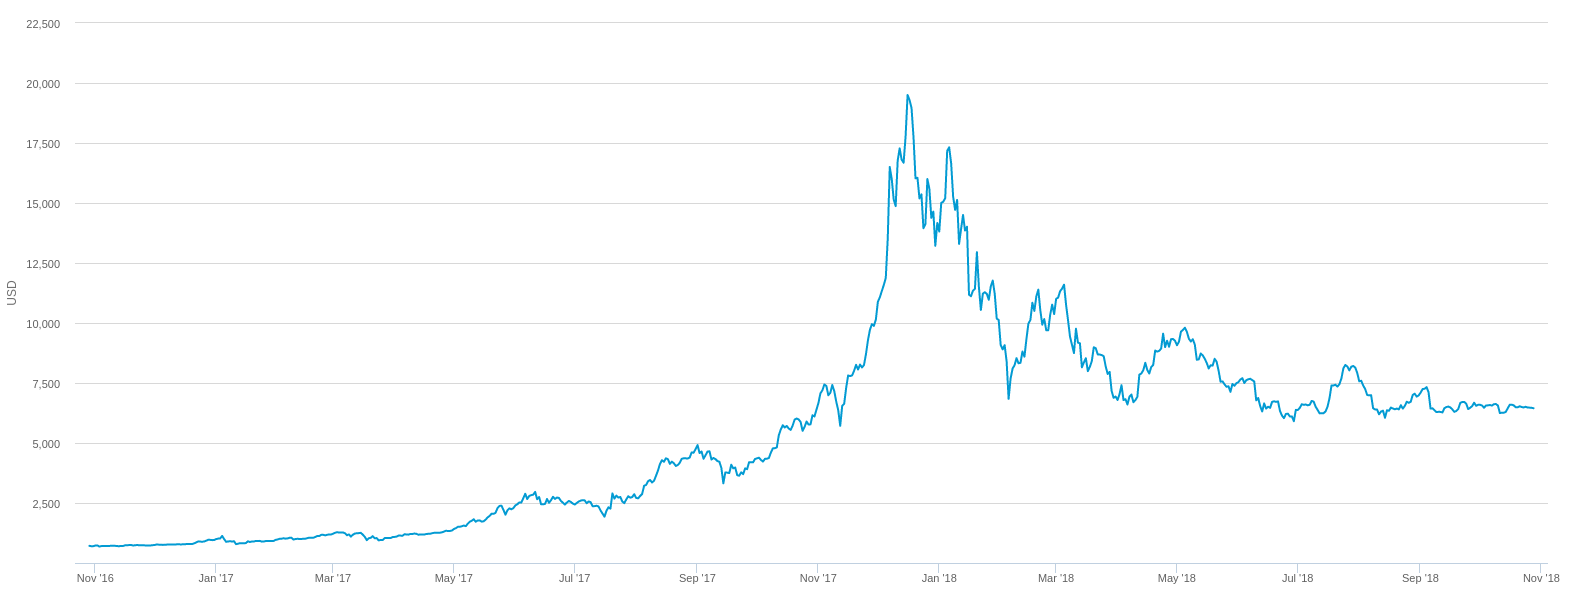
\includegraphics[width=\textwidth]{diagrams/bitcoin-market-price.png}
  \caption[Historical market price of Bitcoin.]{Historical market price (in
  USD) of Bitcoin across major exchanges (Source:~\url{https://blockchain.com}).}
\label{fig:volatility}
\end{figure}

Cryptocurrencies generally fail to achieve the required stability to serve as a
reasonable unit of measurement (Figure~\ref{fig:volatility}).  The volatility
of cyptocurrencies is caused by a combination of a lack of institutions that
could intervene to dampen fluctuations and a comparatively limited liquidity
in the respective
markets.  The latter is exacerbated by the limited ability of decentralized
cryptocurrencies to handle large transaction volumes, despite their extreme
levels of resource consumption.  As a result, the utility of decentralized
cryptocurrencies is limited to highly speculative investments and to the
facilitation of criminal transactions.

With respect to privacy, completely decentralized cryptocurrencies
provide either too much or too little anonymity.  Transparent
cryptocurrencies create the spectre of discriminatory pricing, while
especially for privacy-enhanced cryptocurrencies the lack of
regulation creates an attractive environment for fraud and criminal
activity from tax evasion to financing of terrorism.

These problems are easily addressed by combining the register (or
ledger) with a central bank providing a regulatory framework and
monetary policy, including anti-money-laundering and
know-your-customer enforcement.

\section{Electronic Payments}

Day-to-day payments using registers are expensive and inconvenient.
Using a register requires users to {\em identify} themselves to {\em
  authorize} transactions, and the use of register-based banking
systems tends to be more expensive than the direct exchange of
physical cash.  However, with the ongoing digitalization of daily life
where a significant number of transactions is realized over networks,
some form of electronic payments remain inevitable.

The current alternative to (centrally banked) electronic cash are a
payment systems under full control of oligopoly companies such as
Google, Apple, Facebook or Visa.  The resulting oligopolies are
anti-competitive. In addition to excessive fees, they sometimes even
refuse to process payments with certain types of legal businesses,
which then are often ruined due to lack of alternatives.  Combining
payment services with companies where the core business model is
advertising is also particularly damaging for privacy.  Finally, the
sheer size of these companies creates systemic risks, just as their
global scale creates challenges for regulation.

As GNU Taler is free software, even without backing by a central bank,
Taler would not suffer from these drawbacks arising from the use of
proprietary technology.

Furthermore, Taler-style electronic cash comes
with some unique benefits:
\begin{itemize}
  \item improved income transparency compared to cash and traditional
    Chaum-style e-cash,
  \item anonymity for payers,
  \item avoidance of enticement towards consumer debt --- especially
    compared to credit cards, and
  \item support of new business models and Internet security
    mechanisms which require (anonymous) micro-transactions.
\end{itemize}

Central banks are carefully considering what might be the right
technology to implement an electronic version of their centrally
banked currency, and with Taler we hope to address most of their concerns.
Nevertheless, all electronic payment systems, including Taler even
when backed by central-bank-issued currencies, come with their own
inherent set of risks:~\cite{riksbank2017riksbank}

\begin{itemize}
  \item increased risk of a bank run: in a banking crisis,
    as it is easier to withdraw large amounts of digital
    cash quickly --- even from remote locations;
  \item increased volatility due to foreign holdings that would
    not be as easily possible with physical cash;
  \item increased risk of theft and disruption: while physical
    cash can also be stolen (and likely with much less effort), it is
    difficult to transport in volume~\cite{force2015money}, the
    risk is increased with computers because attacks scale \cite{hammer2018billion}, and
    generally many small incidents are socially preferable over a
    tiny number of very large-scale incidents; and
  \item unavailability in crisis situations without electricity and Internet
    connectivity.
\end{itemize}


We believe that in the case of Taler, some of the risks mentioned
above can be mitigated:
\begin{itemize}
 \item Volatility due to foreign holdings and the resulting increased
   risk of bank runs can be reduced by putting limits on the amount of
   electronic coins that customers can withdraw.  Limiting the
   validity periods of coins is another method that can help
   disincentivize the use of Taler as a value store.
 \item The use of open standards and reference implementations enables
   white-hat security research around GNU Taler, which together with
   good operational security procedures and the possibility of
   competing providers should reduce the risks from attacks.
 \item GNU Taler can co-exist with physical cash, and might even
   help revive the use of cash if it succeeds in reducing credit
   card use online thereby eliminating a key reason for people to
   have credit cards.
\end{itemize}

Unlike cryptocurrencies, Taler does not prescribe a solution for monetary
policy or just taxation, as we believe these issues need to be subject to
continuous political debate and cannot be ``solved'' by simplistic algorithms.
What we offer to society is an open and free (as in free speech) system with
mechanisms to audit merchants' income, instead of proprietary systems
controlled by a few oligopoly companies.
